% kapitel2.tex
\chapter{Basics}
\label{chapter:grundlagen}
\section{Smart Home}
In the course of digitalization and simplification of the procurement of sensor technology in everyday life, smart home has arrived as a concept for the consumer and is affordable. In the most general case, it is a base station with any number of actors and sensors. This station is used to process and store the data from the sensory elements of the network and the actors are then controlled on the basis of decision tables, for example. As a simple scenario, one can imagine a living room lamp that is switched on when the brightness sensor outside signals darkness. However, a system does not necessarily have to have sensors and actors. A network of sensors would only monitor and one of actors can only act. Examples would be a central power consumption monitoring per socket or a heating control.
Here it is worth mentioning that there are also combination devices. A heating thermostat usually has a built-in thermometer and is thus both actor and sensor.\\

\begin{figure}[!h]
	\centering
	\begin{tikzpicture}[every text node part/.style={align=center}]
	\node[] (A) {
\includegraphics[width=50px]{./assets/images/plug-solid}\\Sensor};
	\node[right= 3cm of A] (B) {
\includegraphics[width=50px]{./assets/images/chalkboard-solid}\\Basisstation};
	\node[right= 3cm of B] (C) {
\includegraphics[width=50px]{./assets/images/lightbulb-solid}\\Akteur};
	\draw[-{Stealth[scale=1.3,angle'=90]},semithick] (B) -- node[above] {0..N} (A) ;
	\draw[-{Stealth[scale=1.3,angle'=90]},semithick] (B) -- node[above] {0..M} (C) ;
	\end{tikzpicture}
\end{figure}
\section{Basic Terms}
In the context of Prometheus and this thesis, a few potentially ambiguous terms need to be specified more precisely.
\subsection{Metric}
A property which is observed and measured.
\begin{Beispiel}
	Temperature, rain amount, brightness, transfer rate, amount of printed documents
\end{Beispiel}
\begin{Definition}
	A metric is a single property to be measured.
\end{Definition}
\subsection{Sensor}
A sensor is a real device, a unit which is used in the real world. This can capture multiple metrics and then make them available via an interface.
\begin{Beispiel}
	Weather station, network switch, heating thermostat
\end{Beispiel}
\begin{Definition}
	A metric is a single property to be measured.
\end{Definition}

\section{Prometheus}
Prometheus is an open source solution that is used for metrics monitoring and alerting. There is the possibility to pass data actively or alternatively to configure Prometheus to fetch data from different data sources. For the latter variant, the system to be monitored must provide an HTTP interface on which the data is delivered in a predefined manner. To simplify this process, there are already several libraries for different programming languages that are configurable to such a format. At the time of writing GO, Scala/Java, Python and Ruby are officially supported, but for many other languages there are unofficial third party libraries which are advertised on the Prometheus website. In case the selected language is not supported, it is also possible to create the output yourself. For this, the definition of the output format has been well documented.
\subsection{Metric Types}
Prometheus unterscheidet bei Metriken zwischen verschiedenen Typen. Nachfolgen werden alle Möglichkeiten kurz Erläutern. Im \autoref{subsec:Exportformat}  für das Verständnis ein paar Beispiele aufgelistet und erklärt.
\subsubsection{Counter}
The counter describes a metric type which can only be incremented and reset. It represents a monotonically growing function. 
\subsubsection{Gauge}
This type symbolizes a dial gauge or tachometer. The values can rise and fall.
\subsubsection{Histogram}
A histogram is a concept consisting of so-called buckets. These are initially defined for a metric. With the help of this definition, values of $]-\infty,+\infty[$ are sorted into the said buckets. Each next higher bucket also contains the measured values of the lower bucket. So it is a subset relation where the subsets are determined by the set limit. The \promcode{le} in the index can be interpreted as \textquote{Less Equal}. This parameter is also noted like this in the export.
\begin{center}
	\begin{tikzpicture}
	\draw (0,0) ellipse (2cm and .7cm);
	\draw (2,0) ellipse (4cm and 1cm);
	\draw (4,0) ellipse (6cm and 1.3cm);
	\draw (6,0) ellipse (8cm and 1.5cm);
	\path (0,0) -- (12,0)%
	node[pos=0] {$B_{le=\textquotedbl0.1\textquotedbl}$}%
	node[pos=0.33] {$B_{le=\textquotedbl0.5\textquotedbl}$}%
	node[pos=0.66] {$B_{le=\textquotedbl1\textquotedbl}$}%
	node[pos=1] {$B_{le=\textquotedbl+Inf\textquotedbl}$};
	\end{tikzpicture}
\end{center}
A histogram represents, in addition to the buckets, a total number of measured values, which is like a bucket with \promcode{le="+Inf"} and a value for the sum of all values.
\begin{figure}[hbt!]
	\begin{minted}[mathescape,
	linenos,
	numbersep=5pt,
	gobble=0,
	frame=lines,
	linenos,
	tabsize=4,
	breaklines,
	framesep=2mm]{text}
	# TYPE <basename> histogram
	<basename>_bucket{le="<upper inclusive bound>"} <value>
	<basename>_sum <value>
	<basename>_count <value>
	\end{minted}
	\caption{General concept of histogram export}
\end{figure}
Line 2 can be multiple as long as each entry has its own limit value. Lines 3 and 4 are the additional values as already mentioned.
Zeile 2 kann mehrfach vorhanden sein sofern jeder Eintrag einen eigenen Grenzwert besitzt. Die Zeile 3 und 4 sind wie bereits erwähnt die zusätzlichen Werte.
\subsubsection{Summary}
A summary is similar to a histogram, but here buckets are not filled by the value of the measurement but the measured values are divided into $\varphi$-quantiles ($0 \le \varphi \le 1)$ and the maximum value of the quantile.
\begin{figure}[hbt!]
	\begin{minted}[mathescape,
	linenos,
	numbersep=5pt,
	gobble=0,
	frame=lines,
	linenos,
	tabsize=4,
	breaklines,
	framesep=2mm]{text}
	# TYPE <basename> histogram
	<basename>{quantile="<φ>"} <value>
	<basename>_sum <value>
	<basename>_count <value>
	\end{minted}
	\caption{General concept of summary export}
\end{figure}
\subsubsection{Untyped}
In this case a value is assigned to the metric without following any special rules. This is a safe default setting and it is inevitable not to use this type.
\Needspace{9\baselineskip}
\subsection{Labels}
Labels can be used to break down metrics with the same name into different origins. 
\begin{figure}[!ht]
	\begin{minted}[mathescape,linenos,numbersep=5pt,gobble=1,frame=lines,tabsize=4,breaklines,framesep=2mm]{text}
	<basename>{key="<value>",key2="<value2>",...} <value>
	\end{minted}
	\caption{General concept of labels}
\end{figure}
\subsection{Exportformat}
The export format of Prometheus can be described well by means of an example. For this purpose, we draw a part from the official documentation~\cite{PrometheusExpositionFormatBeispiel}.\\
\par
\label{subsec:Exportformat}
\begin{listing}[H]
	\begin{minted}[mathescape,linenos,numbersep=5pt,gobble=0,frame=lines,linenos,tabsize=4,breaklines,framesep=2mm]{text}
	# HELP http_requests_total The total number of HTTP requests.
	# TYPE http_requests_total counter
	http_requests_total{method="post",code="200"} 1027 1395066363000
	http_requests_total{method="post",code="400"}    3 1395066363000
	
	# Minimalistic line:
	metric_without_timestamp_and_labels 12.47
	\end{minted}
	\caption{Partial example from the official Prometheus documentation~\cite{PrometheusExpositionFormatBeispiel}}
\end{listing}
Between lines 1-4 we find the first exported metric in this example. The first line contains after the token \promcode{# HELP <name of metric>} a short description which is Optional. The next line specifies the type with \linebreak \promcode{# TYPE <name of metric> <type of metric>}. The choices regarding the type coincide with the metric types already described: \promcode{counter}, \promcode{gauge}, \promcode{histogram}, \promcode{summary}, \promcode{untyped}.

All lines starting with \promcode{#} but not continued with \promcode{TYPE} or \promcode{HELP} are comment lines and therefore not interpreted.

Lines 3-4 show the measured values broken down by their labels. Lines that symbolize the measured values consist of three columns. The first in the format \promcode{<name of metric>} followed by optional labels in curly brackets. The example here breaks down all HTTP requests by method and HTTP return value. The next column contains the measured value for the metric, taking into account the optional grouping available. The last column is again non-mandatory and contains the timestamp at which the value was measured. 
In addition, we have a minimal example in line 7. Due to the lack of type specification, the type is \promcode{untyped}. The EBNF to this type of line is as follows:
\begin{listing}[H]
	\begin{samepage}
		\begin{minted}[mathescape,
		linenos,
		numbersep=5pt,
		gobble=1,
		frame=lines,
		linenos,
		tabsize=4,
		breaklines,
		framesep=2mm]{ebnf}
		metric = metric_name, [ 
		"{",
		label_name, "=", '"', label_value, '"',
		{ ",", label_name, "=", '"', label_value, '"' }, [ "," ], 
		"}",
		],  value,  [ timestamp ];
		\end{minted}
		\caption{EBNF following ISO/IEC 14977 of a Metric}
	\end{samepage}
\end{listing}

In the following lines you can see a more complex example. This is a histogram. The values measured internally in the exporter are divided into so-called buckets. You can see the four preconfigured buckets with the limits \promcode{0.05}, \promcode{0.2}, \promcode{1} and \promcode{+Inf}. 
\begin{listing}[H]
	\begin{minted}[mathescape,linenos,numbersep=5pt,gobble=1,frame=lines,tabsize=4,breaklines,framesep=2mm]{text}
	# HELP http_request_duration_seconds A histogram of the request duration
	# TYPE http_request_duration_seconds histogram
	http_request_duration_seconds_bucket{le="0.05"} 24054
	http_request_duration_seconds_bucket{le="0.2"} 100392
	http_request_duration_seconds_bucket{le="1"} 133988
	http_request_duration_seconds_bucket{le="+Inf"} 144320
	http_request_duration_seconds_sum 53423
	http_request_duration_seconds_count 144320
	\end{minted}
	\caption{Histogram export example from the official Prometheus documentation~\cite{PrometheusExpositionFormatBeispiel}}
\end{listing}

\subsection{Prometheus Query Language}
As mentioned before, the collected data is stored in an internal Time Series database which can be searched by the so-called \gls{promql}.

There are four different subtypes for this:
\begin{itemize}
	\item Instant vector
	Instant vector selectors allow the selection of a set of time series and a single sample value for each at a given timestamp (instant): in the simplest form, only a metric name is specified. This results in an instant vector containing elements for all time series that have this metric name.
	%	http_requests_total{job="prometheus",group="canary"}
	
	
	=: Select labels that are exactly equal to the provided string.
	!=: Select labels that are not equal to the provided string.
	=~: Select labels that regex-match the provided string.
	!~: Select labels that do not regex-match the provided string.
	
	
	
	\item Range vector
	%	http_requests_total{job="prometheus"}[5m]
	
	<TimeUnit> ::=
	ms - milliseconds
	s - seconds
	m - minutes
	h - hours
	d - days - assuming a day has always 24h
	w - weeks - assuming a week has always 7d
	y - years - assuming a year has always 365d
	
	%	sum(http_requests_total{method="GET"} offset 5m) // GOOD.
	
	\item Scalar
	[-+]?(
	[0-9]*\.?[0-9]+([eE][-+]?[0-9]+)?
	| 0[xX][0-9a-fA-F]+
	| [nN][aA][nN]
	| [iI][nN][fF]
	)
	23
	-2.43
	3.4e-9
	0x8f
	-Inf
	NaN
	\item String
	"text"
	'test
\end{itemize}

\subsubsection{Arithmetik}

Basistypen:

\begin{bnf*}
	\bnfprod{String}{\bnfts{\textquotedbl...\textquotedbl}\bnfor{}\bnfts{\textquotesingle...\textquotesingle}\bnfor{}\bnfts{`...`}}\\
	\bnfprod{Scalar}{\bnfpn{float}\bnfor\bnfts{nan}\bnfor\bnfts{inf}}\\
	\bnfmore{\bnfor\bnfpn{Scalar}\bnfsp\bnfpn{BinOP}\bnfsp\bnfpn{Scalar}}\\
	\bnfprod{InstantVector}{\bnfpn{identifier}}\\
	\bnfmore{\bnfor\bnfpn{identifier}\bnfsp\bnfts{\{}\bnfsp\bnfpn{InstantVectorProp}\bnfsp\bnfts{\}}}\\
	\bnfmore{\bnfor\bnfpn{InstantVector}\bnfsp\bnfpn{BinOP}\bnfsp\bnfpn{Scalar}}\\
	\bnfprod{InstantVectorProp}{\bnfpn{key}\bnfsp\bnfts{=}\bnfsp\bnfpn{String}}\\
	\bnfmore{\bnfor\bnfpn{key}\bnfsp\bnfts{=}\bnfsp\bnfpn{String}\bnfsp\bnfts{,}\bnfsp\bnfpn{InstantVectorProp}}\\
	\bnfprod{RangeVector}{}\\
	\bnfprod{Scalar}{\bnfpn{Scalar}\bnfsp\bnfpn{BinOP}\bnfsp\bnfpn{Scalar}}\\
	\bnfprod{TimeUnit}{\bnfts{ms}\bnfor\bnfts{s}\bnfor\bnfts{m}\bnfor\bnfts{h}\bnfor\bnfts{d}\bnfor\bnfts{w}\bnfor\bnfts{y}}\\
\end{bnf*}
\begin{bnf*}
	\bnfprod{BinOP}{\bnfts{+} \bnfor \bnfts{-} \bnfor \bnfts{*} \bnfor \bnfts{/} \bnfor \bnfts{\%} \bnfor \bnfts{\textasciicircum}}\\
	\bnfprod{BinCompOP}{\bnfts{==} \bnfor \bnfts{!=} \bnfor \bnfts{>} \bnfor \bnfts{<} \bnfor \bnfts{>=} \bnfor \bnfts{<=}}\\
	\bnfprod{SetOP}{\bnfts{and} \bnfor \bnfts{or} \bnfor \bnfts{unless}}\\
	\bnfprod{InstantVectorPropOP}{\bnfts{=} \bnfor \bnfts{!=} \bnfor \bnfts{=~} \bnfor \bnfts{!~}}
\end{bnf*}

Vector matching 
One-to-one vector matches 
vector1 <operator> vector2
<vector expr> <bin-op> ignoring(<label list>) <vector expr>
<vector expr> <bin-op> on(<label list>) <vector expr>

Many-to-one and one-to-many vector matches 
%<vector expr> <bin-op> ignoring(<label list>) group_left(<label list>) <vector expr>
%<vector expr> <bin-op> ignoring(<label list>) group_right(<label list>) <vector expr>
%<vector expr> <bin-op> on(<label list>) group_left(<label list>) <vector expr>
%<vector expr> <bin-op> on(<label list>) group_right(<label list>) <vector expr>



Aggregation operators 
sum (calculate sum over dimensions)
min (select minimum over dimensions)
max (select maximum over dimensions)
avg (calculate the average over dimensions)
group (all values in the resulting vector are 1)
stddev (calculate population standard deviation over dimensions)
stdvar (calculate population standard variance over dimensions)
count (count number of elements in the vector)
%count_values (count number of elements with the same value)
bottomk (smallest k elements by sample value)
topk (largest k elements by sample value)
%quantile (calculate φ-quantile (0 ≤ φ ≤ 1) over dimensions)

<aggr-op> [without|by (<label list>)] ([parameter,] <vector expression>)
<aggr-op>([parameter,] <vector expression>) [without|by (<label list>)]

Binary operator precedence 
%^
*, /, %
+, -
==, !=, <=, <, >=, >
and, unless
or

\subsubsection{Funktionen}

abs()
absent()
%absent_over_time()
ceil()
changes()
%clamp_max()
%clamp_min()
%day_of_month()
%day_of_week()
%days_in_month()
delta()
deriv()
exp()
floor()
%histogram_quantile()
%holt_winters()
hour()
idelta()
increase()
irate()
%label_join()
%label_replace()
ln()
log2()
log10()
minute()
month()
%predict_linear()
rate()
resets()
round()
scalar()
sort()
%sort_desc()
sqrt()
time()
timestamp()
vector()
year()
%<aggregation>_over_time()

\section{Grafana}
For the visualization of the data collected by Prometheus, Grafana~\citep{GrafanaHomepage} can be used. It is a versatile and extensible system to display data from various data sources like databases like Cassandra, MariaDB or PostgreSQL but also regular HTTP requests against external interfaces or static JSON objects are possible~\cite{GrafanaDataSources}. Furthermore, Grafana also provides different types of diagrams.

\begin{figure}[ht]
	\begin{subfigure}{.25\textwidth}
		\centering
		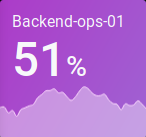
\includegraphics[width=.8\linewidth]{assets/screenshots/Screenshot_2020-12-08 1 - New Features in v7 0 - Grafana.png}
		\captionsetup{justification=centering}
		\caption{Single Metric\\with Graph}
		\label{fig:sfig1}
	\end{subfigure}%
	\begin{subfigure}{.25\textwidth}
		\centering
		
\includegraphics[width=.8\linewidth]{assets/screenshots/Screenshot_2020-12-08 Website trends - Grafana.png}
		\captionsetup{justification=centering}
		\caption{Single Metric\\as Gauge}
		\label{fig:sfig2}
	\end{subfigure}%
	\begin{subfigure}{.5\textwidth}
		\centering
		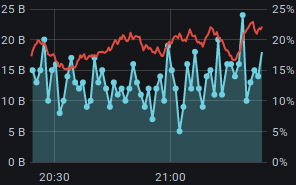
\includegraphics[width=.8\linewidth]{assets/screenshots/Screenshot_2020-12-08 Grafana Play Home - Grafana(2).png}
		\captionsetup{justification=centering}
		\caption{Multimetric plot}
		\label{fig:sfig2}
	\end{subfigure}
	\caption{Example diagram types}
	\label{fig:fig}
\end{figure}
Supplementary there is a simple table format, honeycomb patterns, bar charts and many more. These, like the data sources, are extensible through plugins. Thanks to the source code openness of the project, custom plugins can be written if needed.

To fill the diagrams with data from, in our case, Prometheus, a \gls{promql} query must be stored in each diagram, which is executed regularly. Such a diagram is part of a so-called panel. That means, a panel has exactly one diagram and vice-versa. These are now combined into dashboards, which then provide an overview. Here you can define a lot of panels to display them at the same time.

It should also be said that there are higher order structures such as organizations or you can summarize dashboards again in playlists and / or groups. These features are not considered in this work however more near.

\subsection{Panels}
Since panels have many settings and thus allow many individualizations, these are briefly explained here.

Each panel has primarily a name, description, diagram type, settings for the layout and value reference of cumulative functions and behavior with zero values. Depending on the selected chart type, different configurations are possible. Axis labeling, legend, limits for symbolic coloring and other specific settings.

Alternatively to the grouping of metrics possible by keywords, it is possible to display several metrics in one diagram by specifying several \gls{promql} queries.


